\documentclass[11pt]{article} 
\usepackage{deauthor,times,graphicx}%,hyperref} 

\begin{document}
\title{The Battle for Data Science}
\author{Jeffrey D. Ullman\\Stanford University, Dept.\ of Computer Science\\ullman@gmail.com}

%\maketitle

\section{Introduction}

Through the years, the database community has periodically looked at developments in technology and engaged in hand-wringing over the idea that we are becoming irrelevant.  The cry ``have we missed the boat~-- again'' is common; e.g., here is a panel I served on several years ago \cite{boat}.
My goal in this essay is to argue that the database field and the techniques that have come from this research are still essential for ``data science,'' that is, for the exploitation of data to solve problems of importance in application fields~-- science, commerce, medicine and such.  I believe, as I assume most readers of this article believe, that the field of database systems has always had at its core the study of how to deal with the largest amounts of data possible at the time, whether that be megabytes of corporate payroll data, terabytes of genomic information, or petabytes of satellite output.  Thus whatever study of data is necessary at the time~-- that's our job.

To advance this argument, I want to look at three issues:

\begin{enumerate}

\item
Is the field of statistics really the essential ingredient in data science?

\item
Is machine learning really what data science is all about?

\item
Is data science a danger to decent societal norms?

\end{enumerate}
Hint: my answer to all three is ``no.''  I'll try to address each of these in turn.

\section{The Battle Line: Venn Diagrams for Data Science}

Several years ago, I was invited to a panel of the National Research Council called the ``Data-Science-Education Roundtable.''  The output of this group can be seen at \cite{dsr}.  It was organized not by the computer-science wing of the NRC but the statistics branch.  The participants were roughly equally divided between  statisticians and computer scientists, plus a few from other disciplines.  Part of my experience was seeing how statisticians thought about the world of data and its application.  The most obvious point was that the field of statistics views data science as its own.

To be fair, let's be clear at the outset that I have great respect for statisticians and the work they do.
Statistics has become increasingly important to the modern study of data, including, but not limited to machine learning.
Many statisticians are starting to focus on computation and data analysis in the same way as we do in the database community or in
computer science more generally.  Just to offer one small example, one of my favorite techniques is locality-sensitive hashing, which is an
idea that came squarely out of the database community \cite{lsh}.   Yet one of my colleagues in the Statistics Department at Stanford, Art Owen,
showed me something \cite{owen} about a key step, minhashing \cite{minhash}, that speeds up the process by a very large factor -- something we should have been able to figure out years ago, but didn't.

However, my experience in the roundtable also gave me the sense that there is an effort on the part of some in the statistics community to define statistics as the central component of data science.  I, in contrast, would see the algorithms and techniques for processing large-scale data efficiently as the center of data science.  There is a general sense that data science is a discipline that combines the knowledge of several fields, and I agreed completely.  But what are those fields, and how do they interact?  The question is considered so important that competing communities have published Venn diagrams to justify their own centrality in data science.  There was a recent article \cite{venn} summarizing and commenting upon  a number of these diagrams.  Or if you really want to see the full spectrum of viewpoints expressed as venn diagrams, issue the search query [wikipedia data science venn diagrams].

\subsection{The Conway Diagram}

It appears that statisticians all use a particular diagram, due to Drew Conway.  This diagram shows three sets intersecting: ``hacking skills,'' ``math and statistics,'' and ``substantive expertise.''  At the roundtable, this diagram was shown several times to illustrate the importance of statistics, and I have seen statisticians in several other contexts showing the same diagram to explain the importance of their field to data science.  I reproduce the diagram in Fig.~\ref{drew-diagram-fig}, but I have added my own edits and comments to explain what is misleading about the diagram.

\begin{figure}[h]
\centerline{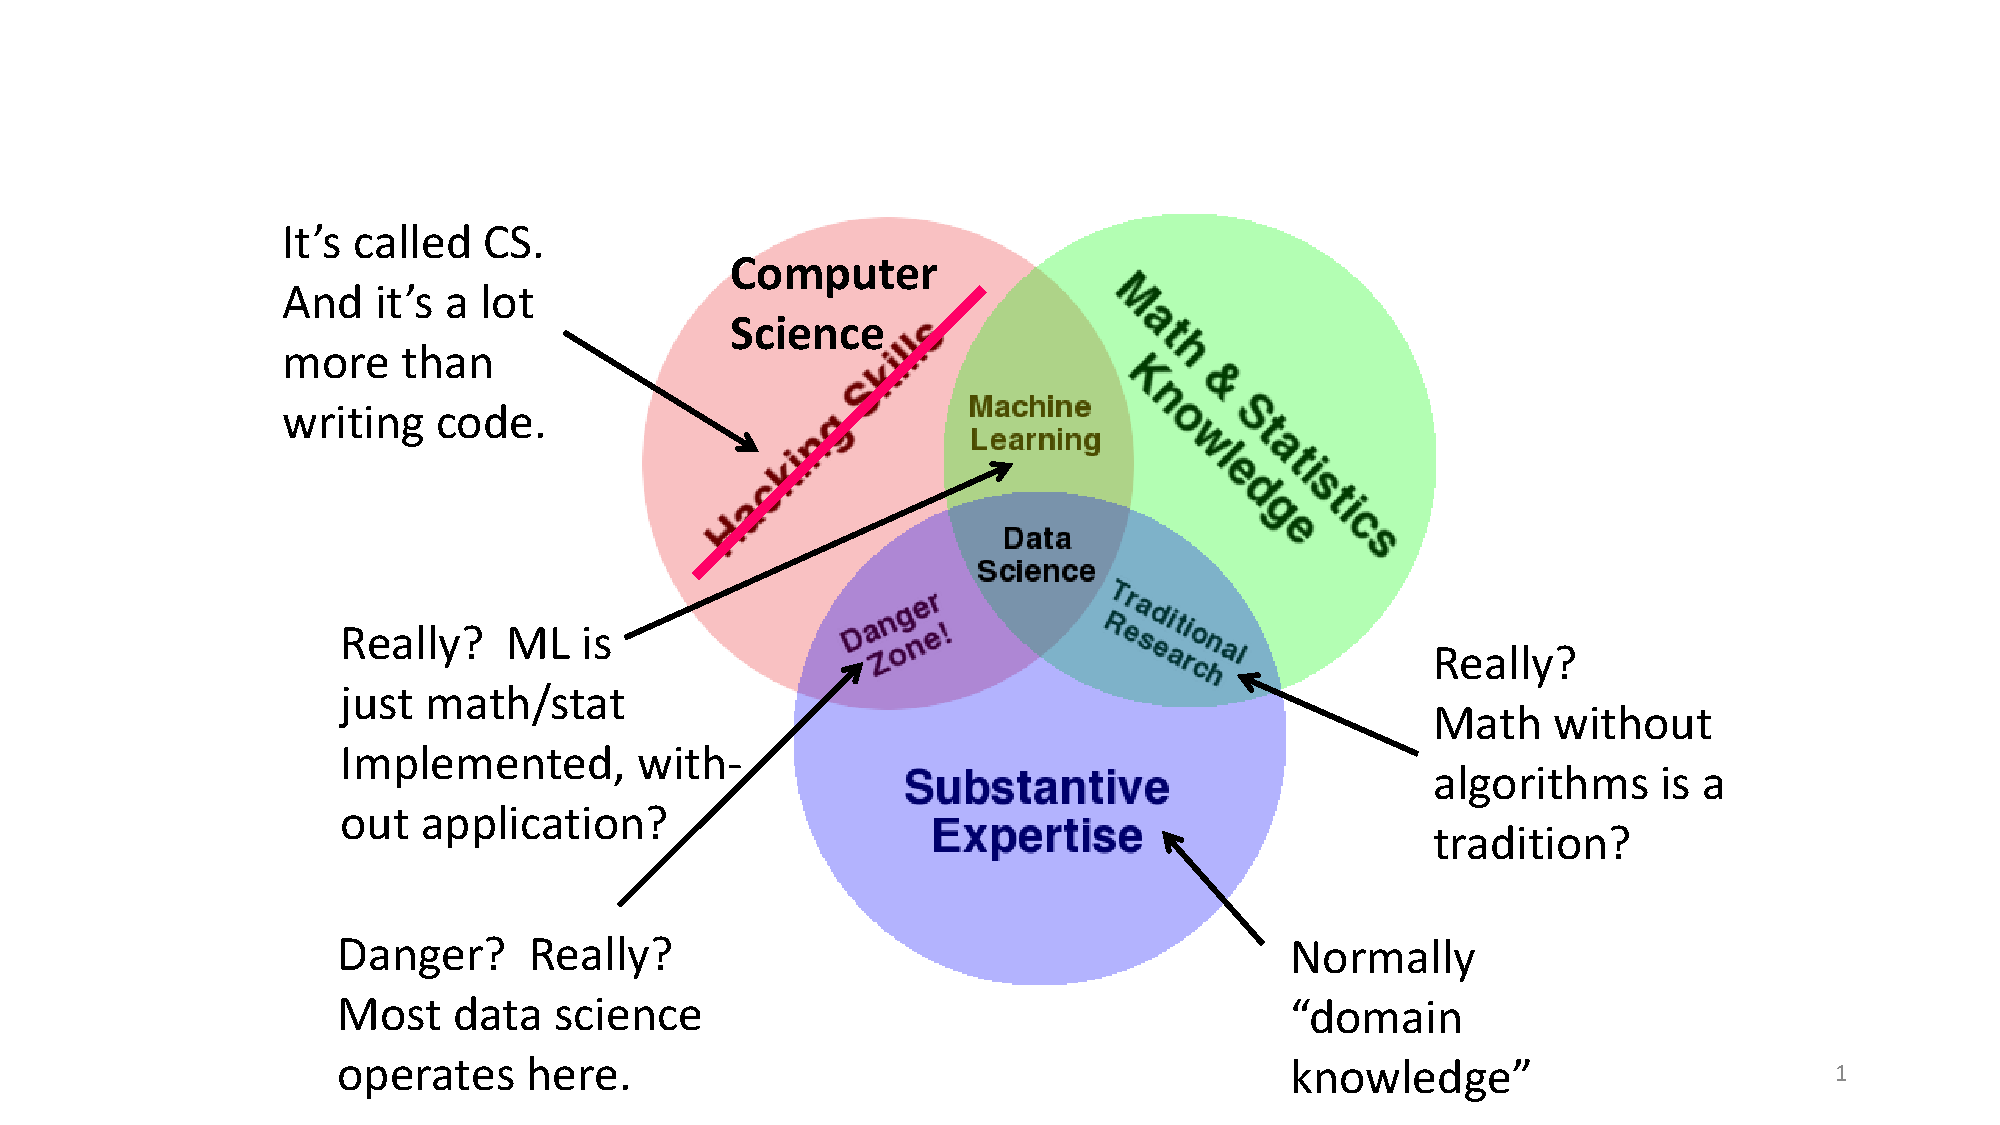
\includegraphics[width=0.8\textwidth]{letters/drew-diagram.pdf}}
\caption{The Conway Venn diagram for data science}
\label{drew-diagram-fig}
\end{figure}

In fact, almost every region of the diagram is misleading in some way.

\begin{enumerate}

\item
First, a small matter: what is referred to as ``substantive expertise'' is generally called ``domain knowledge'' or something similar.

\item
The most egregious impropriety is referring to computer science as ``hacking skills.''  Computer science brings far more to data science than the ability to write code.  We offer algorithms, models, and frameworks, for solving problems of all sorts.  All of that is essential in dealing with data.

\item
``Traditional research'' is shown in the diagram as math/stat intersected with applications.  In other words, in this form of research, one thinks about the application, but does not write any code, and therefore there is nothing that affects the real world.  I don't know whose tradition that is, but I am glad to say it is not the tradition of the database community.

\item
Machine learning has an odd place in this diagram.  It is described as ``hacking'' plus math/stat.  The implication is that machine learning has nothing to do with applications.  In practice, it has everything to do with applications, which is why today the algorithms from machine learning are taken so seriously, not only in the database community, but all across computer science.

\item
And then there is what Conway calls the ``danger zone''~-- writing code to solve problems in application areas without the wise guidance of a statistician.  Well almost all of data science is like that.  For just one example, Google and other mail services are pretty good at detecting phishing emails.  How good?  We really don't know, and even if we could do a statistical analysis today, it would not be valid tomorrow, as the threats change.  The real danger would be refusing to do the best we could, and letting some poor soul send their life savings to some scam artist.

\end{enumerate}

\subsection{My Venn Diagram}

I too offered a Venn diagram (Fig. \ref{myvenn-fig}) that I believe better represents the relationships between the fields.  There is computer science and the various domain sciences, and somewhere in the intersection of these is data science.  Machine learning is a branch of computer science~-- a very important subset these days.  Some of machine learning is used for data science, although there are other uses of machine learning that are more internal to computing.  Many of these applications are considered ``artificial intelligence'' these days, e.g., driverless cars or intrusion detection.  Finally, I see both math and statistics as very important tools for all of computer science, and the small bubbles in my diagram do not do justice to their importance.  However, I drew them as shown to emphasize that they do not really impact domain sciences directly.  but rather they do so through the software that is developed, often with their important aid.

\begin{figure}[h]
\centerline{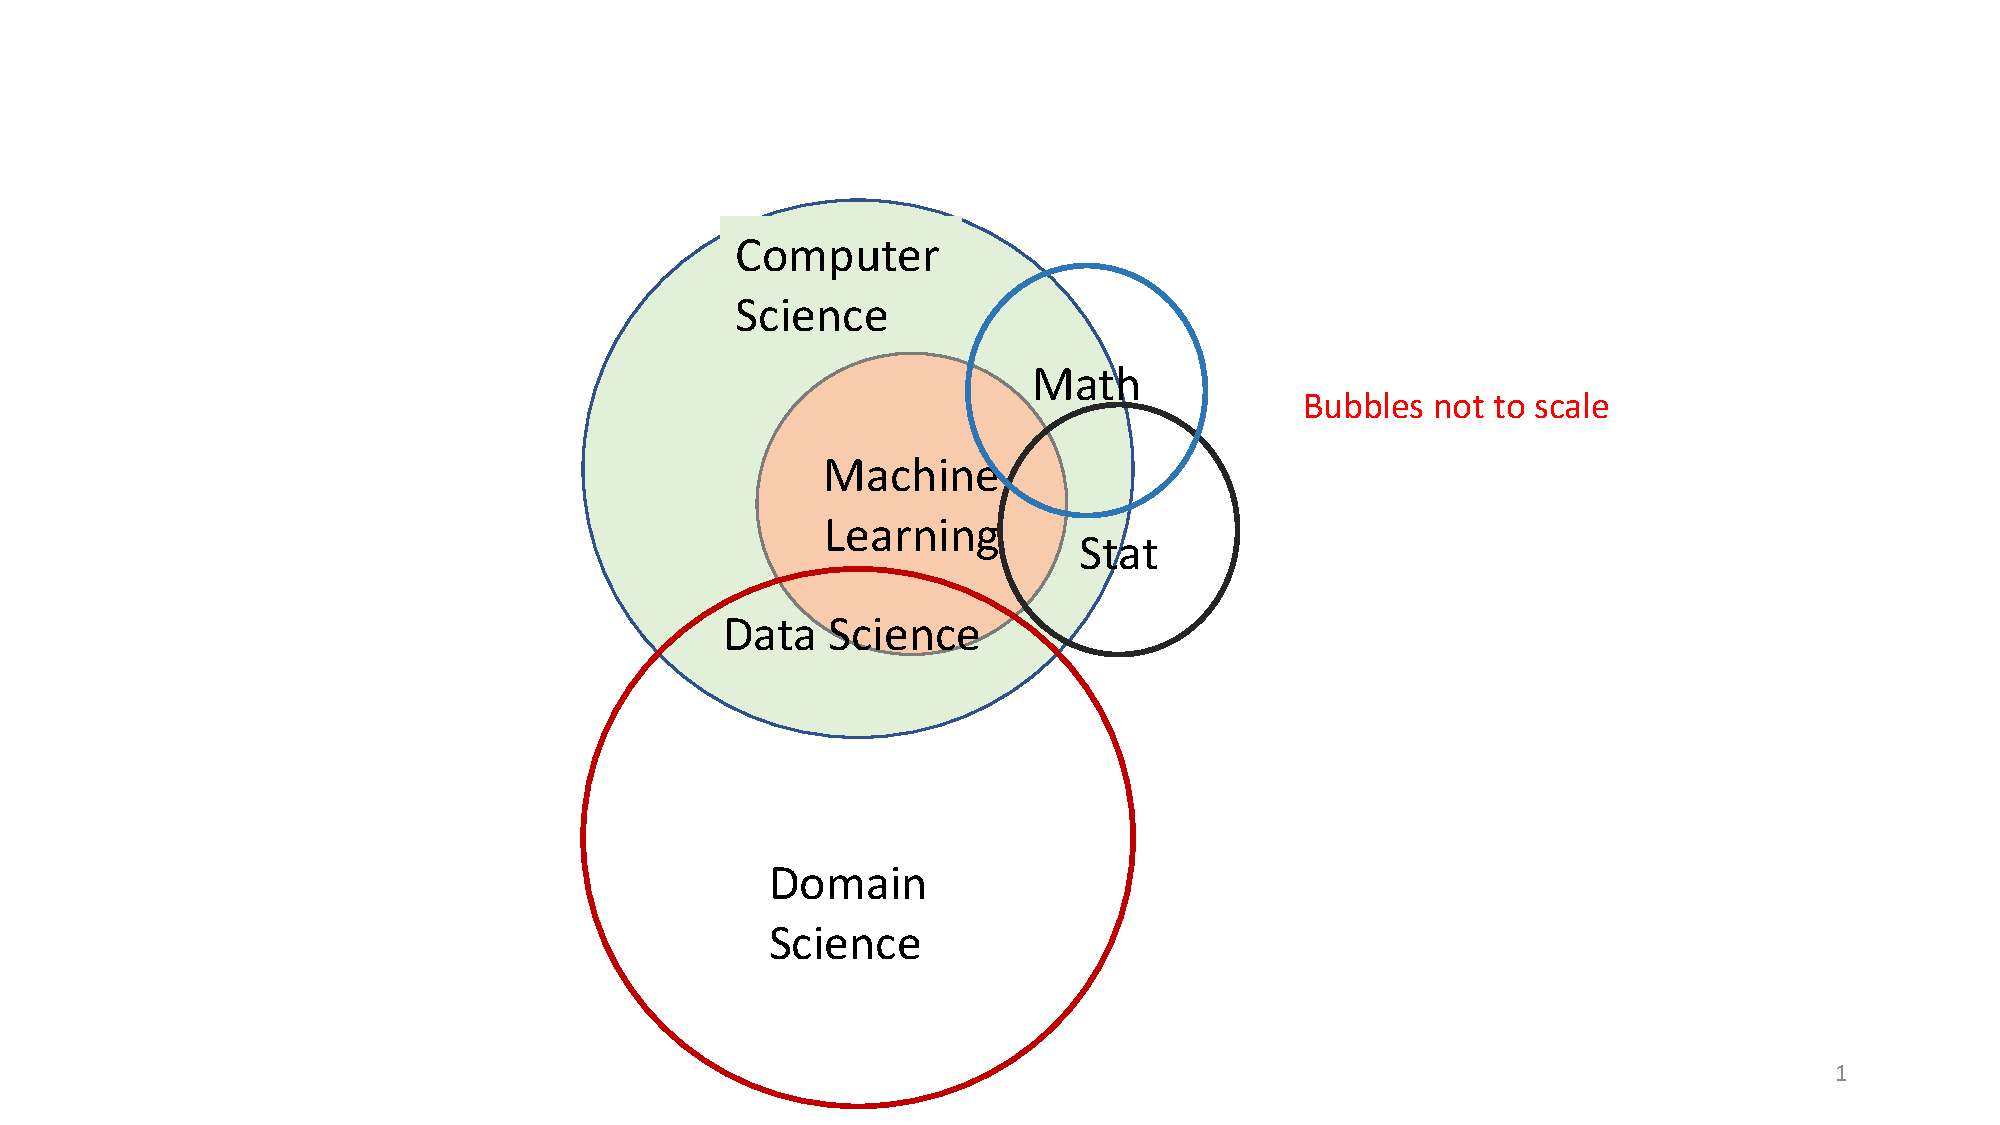
\includegraphics[width=0.8\textwidth]{letters/myvenn.pdf}}
\caption{A personal view of the relationship between computer science, machine learning, and statistics}
\label{myvenn-fig}
\end{figure}

\subsection{The Big Difference: Database and Statistics Value Systems}

Perhaps the most contentious implication of my diagram is that math/stat does not address domain applications directly.  After all, the Conway diagram talks about ``traditional research'' as doing just that.  But while there may be interaction between applications and math/stat that bypasses computing, I think it is rare that the interaction results in any benefit to the application.

To illustrate the distinction, look at the report of the fourth meeting of the data-science education roundtable \cite{datafest}.  One part of the discussion centered on the ``hackathon'' run by the American Statistical Association, called ``Datafest.''  Superficially, this event is just like the sort of hackathon we see run for computer-science students.  The competing teams are given a large dataset, drawn from some application area.  But there is a big difference in how the competition is evaluated.  Competitors are not expected to solve someone's problem, and are not evaluated on the quality of their solution.  Rather, ``awards were given for best data visualization, best use of external data, and best insight.''  In other words, you win a statistical hackathon by doing something of interest to statisticians, not by solving someone else's problem.  I hope the reader appreciates the opposite approach, where the goal is to serve, not to amuse oneself.  That approach, for example, is what drives the computer-science-oriented Kaggle competitions \cite{kaggle}.

\section{Database Systems and Machine Learning}

Now, let us turn to how the rise of machine learning has impacted the use of data.  There is no question that machine learning has had enormous impact on our ability to use data to solve problems.  Many of the most impressive recent achievements have been applications of algorithms in the machine-learning class.  However, I do not believe that machine learning is a complete replacement for the algorithms that have been developed in the database community.  I wish the reader to consider three issues:

\begin{enumerate}

\item
There are many problems involving ``big data'' that are not really machine-learning problems.

\item
Not everything that machine learning claims as its own really comes from there.

\item
Many machine-learning methods produce mysterious models that do not support explanation or justification.

\end{enumerate}

\subsection{Machine Learning Is Not All of Data Science}

I believe a fair definition of machine learning is algorithms that use data to create a model of something, from which answers can be derived.  For example, machine learning can be used to build a model of spam emails, so that a given email can be fed to the model and reliably found to be spam or not spam (``ham'').  But not every useful solution can be expressed as a model.  For example, we earlier mentioned locality-sensitive hashing (LSH) as an important technique from the database community for dealing with data.  LSH is a body of techniques (see, e.g., Chapter 3 of \cite{mmds}) for finding similar items in a dataset without having to look at all pairs.  You don't need for the dataset to be very large before looking at all pairs is prohibitive; even a million items in your set implies half a trillion pairs that would need to be looked at.  So when applicable, LSH can be a very powerful tool.  But there is no model involved.  It is not an instance of machine learning.

\subsection{Machine-Learning Advocates Sometimes Claim Too Much}

I have heard of clustering, for example, defined as a branch of machine learning, even though clustering has been studied from well before there was such a thing as machine learning.  Gradient descent is another example of something that predates machine learning, yet somehow is popularly regarded as a machine-learning topic.  Another important example concerns {\em association rules}.  This idea was pioneered in 1993--4 by Rakesh Agrawal and his friends \cite{ais} \cite{as} and predates almost all of machine learning.   I even recall talking to a machine-learning advocate and offering LSH as an example of a big-data algorithm that had nothing to do with machine learning.  His response was that LSH ``must be machine learning, because it is a really good idea.''

\subsection{Explainability}

Often, a machine-learning algorithm draws correct conclusions that cannot be explained except by showing the model.  And that model is often so complex that it means nothing to the average user.  Sometimes, no one cares; the important thing is that the model, say, gives the correct diagnosis, even if its reasoning is hidden in the processing of a megapixel image.  On the other hand, sometimes, we have a right to an explanation.  For example, if your insurance company raises your rates because some model of automobile accidents has decided you are more likely to have an accident than the previous model showed, it seems proper that you at least be told why this is happening to you.  In Europe, the GDPR laws \cite{gdpr} guarantee you that right.

But non-machine-learning approaches are often more explainable than machine-learning models.  To see the difference, let us reconsider the matter of association rules as a way to identify spam emails.  One would produce a set of ``rules,'' which in this case would be sets of words, whose presence in an email indicates it is spam.  You might think of these rules as a model of spam, which is probably why machine-learning advocates view the method as their own.  But in fact, the algorithms used to find association rules do not ``learn'' a model from the data.  They simply count the number of spam emails that contain certain sets of words, and if that count is high enough, they declare a rule that emails containing that set of words is spam.  For instance, we might expect that one rule would say that emails containing the set $\{${\tt Nigerian}, {\tt prince}$\}$ are spam.  In contrast, even the simplest machine-learning technique, such as learning a (positive or negative) weight on each possible word, and declaring spam if the sum of the weights exceeds a threshold, will be more accurate than a solution based on association rules.

However, the association-rule approach is explainable, while the machine-learning model is not.  If I really {\em am} a Nigerian prince, and all my emails are sent to spam, at least I can understand why.  On the other hand, if you have ever asked gmail why it declared something to be spam, its usual answer is something like ``it looked like other emails that were spam.''  That is, whatever model we are using today said it was spam, and that's all we can tell you.\footnote{Interestingly, I was the victim in way similar to that of the hypothetical Nigerian prince.  A dean asked me for a letter concerning a candidate for promotion, which I sent.  He claimed the email never arrived, so I sent it again.  It never arrived.  Eventually, he discovered that the mail system at his university had a rule that said anything from my email address was to be discarded immediately.  I suspect someone at some time engaged in a denial-of-service attack using my faked email address.  At least we were able to understand the problem and get it fixed quickly.}

\section{Attacks on the Use of Data}

It is common to blame data for the ills of society.  However, the fault rarely lies in the idea of using data to address a social issue.  Rather, the source of error is more likely to come from:

\begin{enumerate}

\item
People intentionally or unintentionally misusing the data, or

\item
Problems in the reality that the data faithfully reflects.

\end{enumerate}

\subsection{Misuse of Data}

At the Data-Science-Education Roundtable, there was a discussion in the fifth session on data ethics, which you may find in \cite{ethics}.  One common problem discussed was the use of ``false proxies.''  For an example given there, a city wants to deploy its police to the areas where crime occurs.  What they have is data on where arrests occur, so they send their police there, and lo and behold, they arrest more from those areas.  But arrests do not reflect solely the occurrence of crime; they also reflect the presence of police to make the arrests.  So a possible error is perpetuated by the data.  That is, if for bad reasons, police had been sent to certain areas preferentially in the past, the data will truly reflect that there are more arrests in those areas.  Perhaps, just as much crime occurs elsewhere, but the arrest rate is lower in places where the police presence is low.

Another common example of where data can perpetuate bias concerns a hypothetical company that has always discriminated against women when promotions are handed out.  They want to build an AI system using machine learning, to process resumes and identify those with characteristics similar to those of their successful employees.  But the data shows that being female is an indication that the candidate will not be successful, so the machine-learning algorithm learns from the data to reject applications from females.   The data again perpetuates an existing bias.  But the data didn't create the bias; people did.

\subsection{Data Reflecting a World We Don't Like}

A less reasonable charge against the use of data is that the resulting systems reflect something about society that the speaker opposes.  A clear example of this sort of false reasoning concerns Word2Vec \cite{word2vec}, a system developed at Google several years ago (since popularly superseded by an alternative system called BERT \cite{bert}) that embeds words in a high-dimensional vector space, in such a way that words with similar meaning have vectors that are close.  The intuitive idea is to look at the words that typically surround the word $w$ in question.  The vector for $w$ then is a weighed combination of directions associated with its surrounding words.  For example, we would expect {\tt Coke} and {\tt Pepsi} to have similar vectors, because people talk about them in much the same way.

The problem arose when it was observed that certain vector equations were approximately followed.  For example, as vectors,

\begin{center}
{\tt London} $-$ {\tt England} + {\tt France} = {\tt Paris}
\end{center}
That is, London and Paris, being the capitals and largest cities of their respective countries, have around them many words reflecting that status.  However, we would expect London to have more words that are associated with England surrounding it, so take them away and substitute words associated with France.

No one was disturbed by that observation, but other equations raised some hackles.  For instance, \cite{buono} called out the equation

\begin{center}
{\tt doctor} $-$ {\tt man} + {\tt woman} = {\tt nurse}
\end{center}
A similar objection to another such equation is discussed in \cite{boluk}.  However, if you look at this equation, it is asking ``find me a profession like doctor, but with more females.  About 50\% of doctors are women, but close to 90\% of nurses are women.  We expect that words surrounding {\tt doctor} and {\tt nurse} would be similar, but the latter will more often be found near words like {\tt she}.  So the equation makes sense.  What these negative articles are really objecting to is a society where women are more likely to be channeled into nursing.  I agree, and probably in the not-too-distant future, that will not be the case.  But my point is: don't blame the data.  Systems like Word2Vec or BERT, when trained on a large corpus like Wikipedia, will reflect language as used by a broad segment of the public, and that usage will in turn reflect what is generally thought to be true, regardless of whether we like that truth or not.

\section{The Last Word}

I hope the reader will take away the following thoughts:

\begin{itemize}

\item
Data and its management is still the essence of data science.

\item
While machine learning is very important, it is far from the only tool or idea needed for effective data science.

\item
Although there have been misuses of data, we should not blame data if it reflects the world as it is, rather than as we would like it to be.

\end{itemize}

\vspace{-.1cm}
\bibliographystyle{ACM-Reference-Format}
\begin{thebibliography}{10}
\begin{small}
\itemsep=-.5pt

\bibitem{ais}
R. Agrawal, T. Imielinski, and A. Swami,
``Mining associations between sets of items in massive databases,''
{\em Proc.\ ACM SIGMOD Intl.\ Conf.\ on Management of Data},
pp.~207--216, 1993.

\bibitem{as}
R. Agrawal and R. Srikant,
``Fast algorithms for mining association rules,''
{\em Intl.\ Conf.\ on Very Large Databases}, pp.~487--499, 1994.

\bibitem{boluk}
T. Bolukbasi, K.-W. Chang, J. Zou, V. Saligrama, and A. Kalai,
``Man is to computer programmer as woman is to homemaker? Debiasing word embeddings,''
{\em 30th Conference on Neural Information Processing Systems}, Barcelona, 2016.

\bibitem{minhash}
A.Z. Broder, M. Charikar, A.M. Frieze, and M. Mitzenmacher,
``Min-wise independent permutations,''
{\em ACM Symposium on Theory of Computing}, pp.~327--336, 1998.

\bibitem{buono}
T. Buonocore, ``Man is to doctor as woman is to nurse: the gender bias of word embeddings,'' https://towardsdatascience.com/gender-bias-word-embeddings-76d9806a0e17

\bibitem{bert}
J. Devlin, M.-W. Chang, K. Lee, and K. Toutanova,
``BERT: Pre-training of deep bidirectional transformers for language understanding,''
arXiv:1810.04805, 2018.

\bibitem{lsh}
A. Gionis, P. Indyk, and R. Motwani,
``Similarity search in high dimensions via hashing,''
{\em Proc.\ Intl.\ Conf.\ on Very Large Databases}, pp.~518--529, 1999.

\bibitem{boat}
B. Howe, M.J. Franklin, L.M. Haas, T. Kraska, and J.D. Ullman:
``Data science education: we're missing the boat, again,'' {\em ICDE}, pp.~1473--1474, 2017.

\bibitem{kaggle}
https://www.kaggle.com/

\bibitem{venn}
https://www.kdnuggets.com/2016/10/battle-data-science-venn-diagrams.html

\bibitem{mmds}
J. Leskovec, A. Rajaraman, and J.D.Ullman,
{\em Mining of Massive Datasets} 3rd edition, Cambridge Univ.\ Press, 2020.  Available for download at http://www.mmds.org

\bibitem{owen}
P. Li, A.B. Owen, and C.H. Zhang.
``One permutation hashing,''
{\em Conf.\ on Neural Information Processing Systems} 2012, pp.~3122--3130.

\bibitem{word2vec}
T. Mikolov, K. Chen, G. Corrado, and J. Dean,
``Efficient estimation of word representations in vector space,''
ArXiv:1301.3781, 2013.

\bibitem{datafest}
https://www.nationalacademies.org/event/10-20-2017/docs/DCE05D1E271C31C585455B25E43AE9E5462ED3312DB2

\bibitem{ethics}
https://www.nationalacademies.org/event/12-08-2017/docs/D8EE65EFC7F4B0C368D267EDAD10E5AB1BAFBE3369D2

\bibitem{dsr}
https://www.nationalacademies.org/our-work/roundtable-on-data-science-postsecondary-education

\bibitem{gdpr}
https://en.wikipedia.org/wiki/Right\_to\_explanation


\end{small}
\end{thebibliography}

\end{document}
